% SOURCE: submissions/d2-neurocomputing/zenodo-deposit/results/merging/RG_gain_holdout_20260716.json :: orderings (full_pooled -0.8227 p=2.61e-6, heldout_split -0.8238); permutation null computed in-script over submissions/d2-neurocomputing/zenodo-deposit/results/merging/RG_gain_law_MERGED_REFIX20260730.json :: bundles.*.{gain_median_absdrop_per_dose,frac_drop_negative} (seed 20260801, 0/20000 draws at threshold)
% !TEX encoding = UTF-8 Unicode
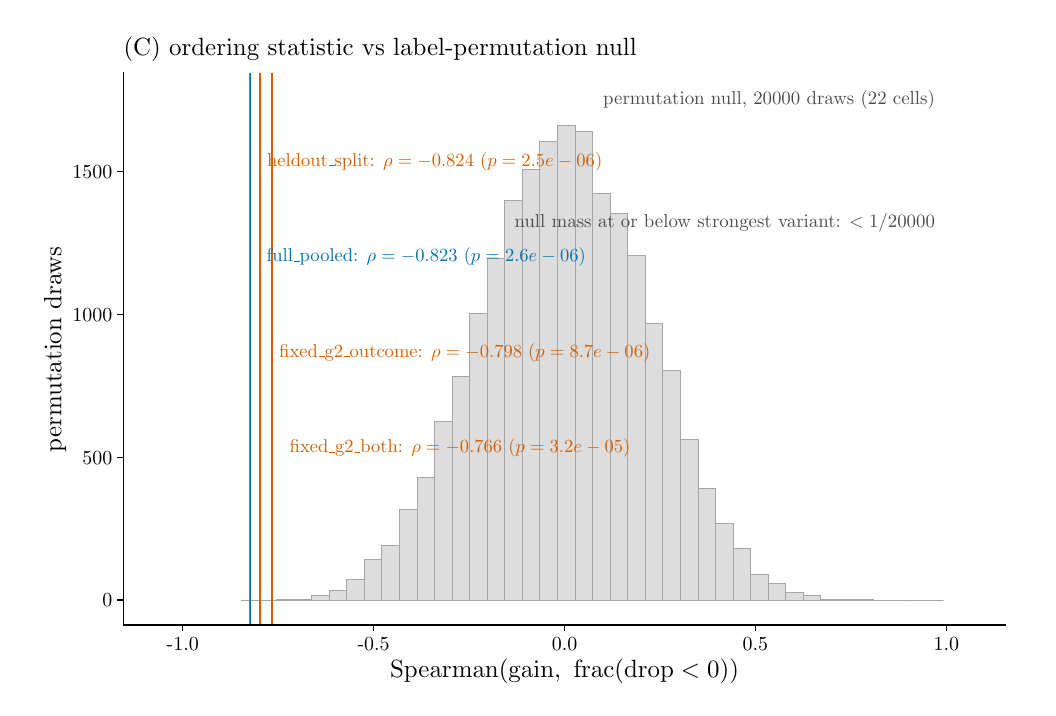
\begin{tikzpicture}[x=1pt,y=1pt]
\definecolor{fillColor}{RGB}{255,255,255}
\path[use as bounding box,fill=fillColor,fill opacity=0.00] (0,0) rectangle (361.35,238.49);
\begin{scope}
\path[clip] (  0.00,  0.00) rectangle (361.35,238.49);
\definecolor{drawColor}{RGB}{255,255,255}
\definecolor{fillColor}{RGB}{255,255,255}

\path[draw=drawColor,line width= 0.5pt,line join=round,line cap=round,fill=fillColor] (  0.00,  0.00) rectangle (361.35,238.49);
\end{scope}
\begin{scope}
\path[clip] ( 34.64, 22.61) rectangle (353.35,222.04);
\definecolor{fillColor}{RGB}{255,255,255}

\path[fill=fillColor] ( 34.64, 22.61) rectangle (353.35,222.04);
\definecolor{drawColor}{gray}{0.65}
\definecolor{fillColor}{RGB}{221,221,221}

\path[draw=drawColor,line width= 0.2pt,fill=fillColor] ( 77.16, 31.67) rectangle ( 83.51, 31.67);

\path[draw=drawColor,line width= 0.2pt,fill=fillColor] ( 83.51, 31.67) rectangle ( 89.85, 31.67);

\path[draw=drawColor,line width= 0.2pt,fill=fillColor] ( 89.85, 31.67) rectangle ( 96.20, 31.77);

\path[draw=drawColor,line width= 0.2pt,fill=fillColor] ( 96.20, 31.67) rectangle (102.55, 31.77);

\path[draw=drawColor,line width= 0.2pt,fill=fillColor] (102.55, 31.67) rectangle (108.89, 33.32);

\path[draw=drawColor,line width= 0.2pt,fill=fillColor] (108.89, 31.67) rectangle (115.24, 35.28);

\path[draw=drawColor,line width= 0.2pt,fill=fillColor] (115.24, 31.67) rectangle (121.58, 39.10);

\path[draw=drawColor,line width= 0.2pt,fill=fillColor] (121.58, 31.67) rectangle (127.93, 46.32);

\path[draw=drawColor,line width= 0.2pt,fill=fillColor] (127.93, 31.67) rectangle (134.28, 51.59);

\path[draw=drawColor,line width= 0.2pt,fill=fillColor] (134.28, 31.67) rectangle (140.62, 64.48);

\path[draw=drawColor,line width= 0.2pt,fill=fillColor] (140.62, 31.67) rectangle (146.97, 76.04);

\path[draw=drawColor,line width= 0.2pt,fill=fillColor] (146.97, 31.67) rectangle (153.31, 96.37);

\path[draw=drawColor,line width= 0.2pt,fill=fillColor] (153.31, 31.67) rectangle (159.66,112.67);

\path[draw=drawColor,line width= 0.2pt,fill=fillColor] (159.66, 31.67) rectangle (166.01,135.16);

\path[draw=drawColor,line width= 0.2pt,fill=fillColor] (166.01, 31.67) rectangle (172.35,155.28);

\path[draw=drawColor,line width= 0.2pt,fill=fillColor] (172.35, 31.67) rectangle (178.70,176.02);

\path[draw=drawColor,line width= 0.2pt,fill=fillColor] (178.70, 31.67) rectangle (185.04,187.37);

\path[draw=drawColor,line width= 0.2pt,fill=fillColor] (185.04, 31.67) rectangle (191.39,197.49);

\path[draw=drawColor,line width= 0.2pt,fill=fillColor] (191.39, 31.67) rectangle (197.73,203.16);

\path[draw=drawColor,line width= 0.2pt,fill=fillColor] (197.73, 31.67) rectangle (204.08,201.20);

\path[draw=drawColor,line width= 0.2pt,fill=fillColor] (204.08, 31.67) rectangle (210.43,178.50);

\path[draw=drawColor,line width= 0.2pt,fill=fillColor] (210.43, 31.67) rectangle (216.77,171.38);

\path[draw=drawColor,line width= 0.2pt,fill=fillColor] (216.77, 31.67) rectangle (223.12,156.11);

\path[draw=drawColor,line width= 0.2pt,fill=fillColor] (223.12, 31.67) rectangle (229.46,131.55);

\path[draw=drawColor,line width= 0.2pt,fill=fillColor] (229.46, 31.67) rectangle (235.81,114.63);

\path[draw=drawColor,line width= 0.2pt,fill=fillColor] (235.81, 31.67) rectangle (242.16, 89.66);

\path[draw=drawColor,line width= 0.2pt,fill=fillColor] (242.16, 31.67) rectangle (248.50, 72.02);

\path[draw=drawColor,line width= 0.2pt,fill=fillColor] (248.50, 31.67) rectangle (254.85, 59.53);

\path[draw=drawColor,line width= 0.2pt,fill=fillColor] (254.85, 31.67) rectangle (261.19, 50.24);

\path[draw=drawColor,line width= 0.2pt,fill=fillColor] (261.19, 31.67) rectangle (267.54, 40.96);

\path[draw=drawColor,line width= 0.2pt,fill=fillColor] (267.54, 31.67) rectangle (273.89, 37.86);

\path[draw=drawColor,line width= 0.2pt,fill=fillColor] (273.89, 31.67) rectangle (280.23, 34.56);

\path[draw=drawColor,line width= 0.2pt,fill=fillColor] (280.23, 31.67) rectangle (286.58, 33.53);

\path[draw=drawColor,line width= 0.2pt,fill=fillColor] (286.58, 31.67) rectangle (292.92, 31.88);

\path[draw=drawColor,line width= 0.2pt,fill=fillColor] (292.92, 31.67) rectangle (299.27, 31.88);

\path[draw=drawColor,line width= 0.2pt,fill=fillColor] (299.27, 31.67) rectangle (305.62, 31.77);

\path[draw=drawColor,line width= 0.2pt,fill=fillColor] (305.62, 31.67) rectangle (311.96, 31.67);

\path[draw=drawColor,line width= 0.2pt,fill=fillColor] (311.96, 31.67) rectangle (318.31, 31.67);

\path[draw=drawColor,line width= 0.2pt,fill=fillColor] (318.31, 31.67) rectangle (324.65, 31.67);

\path[draw=drawColor,line width= 0.2pt,fill=fillColor] (324.65, 31.67) rectangle (331.00, 31.67);
\definecolor{drawColor}{RGB}{213,94,0}

\path[draw=drawColor,line width= 0.5pt,line join=round] ( 80.34, 22.61) -- ( 80.34,222.04);
\definecolor{drawColor}{RGB}{0,114,178}

\path[draw=drawColor,line width= 0.5pt,line join=round] ( 80.49, 22.61) -- ( 80.49,222.04);
\definecolor{drawColor}{RGB}{213,94,0}

\path[draw=drawColor,line width= 0.5pt,line join=round] ( 83.92, 22.61) -- ( 83.92,222.04);

\path[draw=drawColor,line width= 0.5pt,line join=round] ( 88.28, 22.61) -- ( 88.28,222.04);

\node[text=drawColor,anchor=base west,inner sep=0pt, outer sep=0pt, scale=  0.67] at ( 86.52,188.47) {heldout\_split: $\rho=-0.824$ ($p=2.5e-06$)};
\definecolor{drawColor}{RGB}{0,114,178}

\node[text=drawColor,anchor=base west,inner sep=0pt, outer sep=0pt, scale=  0.67] at ( 86.38,153.94) {full\_pooled: $\rho=-0.823$ ($p=2.6e-06$)};
\definecolor{drawColor}{RGB}{213,94,0}

\node[text=drawColor,anchor=base west,inner sep=0pt, outer sep=0pt, scale=  0.67] at ( 90.89,119.41) {fixed\_g2\_outcome: $\rho=-0.798$ ($p=8.7e-06$)};

\node[text=drawColor,anchor=base west,inner sep=0pt, outer sep=0pt, scale=  0.67] at ( 94.70, 84.87) {fixed\_g2\_both: $\rho=-0.766$ ($p=3.2e-05$)};
\definecolor{drawColor}{gray}{0.30}

\node[text=drawColor,anchor=base east,inner sep=0pt, outer sep=0pt, scale=  0.68] at (327.83,210.63) {permutation null, 20000 draws (22 cells)};

\node[text=drawColor,anchor=base east,inner sep=0pt, outer sep=0pt, scale=  0.68] at (327.83,166.22) {null mass at or below strongest variant: $<1/20000$};
\end{scope}
\begin{scope}
\path[clip] (  0.00,  0.00) rectangle (361.35,238.49);
\definecolor{drawColor}{RGB}{0,0,0}

\path[draw=drawColor,line width= 0.5pt,line join=round,line cap=rect] ( 34.64, 22.61) --
	( 34.64,222.04);
\end{scope}
\begin{scope}
\path[clip] (  0.00,  0.00) rectangle (361.35,238.49);
\definecolor{drawColor}{RGB}{0,0,0}

\node[text=drawColor,anchor=base east,inner sep=0pt, outer sep=0pt, scale=  0.72] at ( 30.59, 29.19) {0};

\node[text=drawColor,anchor=base east,inner sep=0pt, outer sep=0pt, scale=  0.72] at ( 30.59, 80.78) {500};

\node[text=drawColor,anchor=base east,inner sep=0pt, outer sep=0pt, scale=  0.72] at ( 30.59,132.37) {1000};

\node[text=drawColor,anchor=base east,inner sep=0pt, outer sep=0pt, scale=  0.72] at ( 30.59,183.97) {1500};
\end{scope}
\begin{scope}
\path[clip] (  0.00,  0.00) rectangle (361.35,238.49);
\definecolor{drawColor}{RGB}{0,0,0}

\path[draw=drawColor,line width= 0.5pt,line join=round] ( 32.39, 31.67) --
	( 34.64, 31.67);

\path[draw=drawColor,line width= 0.5pt,line join=round] ( 32.39, 83.26) --
	( 34.64, 83.26);

\path[draw=drawColor,line width= 0.5pt,line join=round] ( 32.39,134.85) --
	( 34.64,134.85);

\path[draw=drawColor,line width= 0.5pt,line join=round] ( 32.39,186.45) --
	( 34.64,186.45);
\end{scope}
\begin{scope}
\path[clip] (  0.00,  0.00) rectangle (361.35,238.49);
\definecolor{drawColor}{RGB}{0,0,0}

\path[draw=drawColor,line width= 0.5pt,line join=round,line cap=rect] ( 34.64, 22.61) --
	(353.35, 22.61);
\end{scope}
\begin{scope}
\path[clip] (  0.00,  0.00) rectangle (361.35,238.49);
\definecolor{drawColor}{RGB}{0,0,0}

\path[draw=drawColor,line width= 0.5pt,line join=round] ( 56.03, 20.36) --
	( 56.03, 22.61);

\path[draw=drawColor,line width= 0.5pt,line join=round] (125.01, 20.36) --
	(125.01, 22.61);

\path[draw=drawColor,line width= 0.5pt,line join=round] (194.00, 20.36) --
	(194.00, 22.61);

\path[draw=drawColor,line width= 0.5pt,line join=round] (262.98, 20.36) --
	(262.98, 22.61);

\path[draw=drawColor,line width= 0.5pt,line join=round] (331.96, 20.36) --
	(331.96, 22.61);
\end{scope}
\begin{scope}
\path[clip] (  0.00,  0.00) rectangle (361.35,238.49);
\definecolor{drawColor}{RGB}{0,0,0}

\node[text=drawColor,anchor=base,inner sep=0pt, outer sep=0pt, scale=  0.72] at ( 56.03, 13.60) {-1.0};

\node[text=drawColor,anchor=base,inner sep=0pt, outer sep=0pt, scale=  0.72] at (125.01, 13.60) {-0.5};

\node[text=drawColor,anchor=base,inner sep=0pt, outer sep=0pt, scale=  0.72] at (194.00, 13.60) {0.0};

\node[text=drawColor,anchor=base,inner sep=0pt, outer sep=0pt, scale=  0.72] at (262.98, 13.60) {0.5};

\node[text=drawColor,anchor=base,inner sep=0pt, outer sep=0pt, scale=  0.72] at (331.96, 13.60) {1.0};
\end{scope}
\begin{scope}
\path[clip] (  0.00,  0.00) rectangle (361.35,238.49);
\definecolor{drawColor}{RGB}{0,0,0}

\node[text=drawColor,anchor=base,inner sep=0pt, outer sep=0pt, scale=  0.90] at (194.00,  3.75) {Spearman$(\mathrm{gain},\ \mathrm{frac(drop}<0))$};
\end{scope}
\begin{scope}
\path[clip] (  0.00,  0.00) rectangle (361.35,238.49);
\definecolor{drawColor}{RGB}{0,0,0}

\node[text=drawColor,rotate= 90.00,anchor=base,inner sep=0pt, outer sep=0pt, scale=  0.90] at ( 12.20,122.32) {permutation draws};
\end{scope}
\begin{scope}
\path[clip] (  0.00,  0.00) rectangle (361.35,238.49);
\definecolor{drawColor}{RGB}{0,0,0}

\node[text=drawColor,anchor=base west,inner sep=0pt, outer sep=0pt, scale=  0.90] at ( 34.64,228.29) {(C) ordering statistic vs label-permutation null};
\end{scope}
\end{tikzpicture}
